\section{BEE-Charliecloud}
\label{bee-charliecloud-section}
Charliecloud \cite{priedhorsky2016charliecloud} is a Linux container runtime based on Linux user namespaces. It offers all the necessary runtime functionalities for HPC applications. It has three major benefits that make it the ideal runtime for \texttt{BEE} on HPC systems: First, it takes standard Docker images as input via the built-in image flattener, so it helps maintain the same user interface as the other three \texttt{BEE backends}. Second, Linux user namespaces only bring minor performance overhead, full exposure of host hardware resources, and no requirement of privileged operations or daemons. Third, Linux user namespaces is widely supported by default on current HPC systems,  making \texttt{BEE} a highly usable framework. So, using Charliecloud we design \texttt{BEE-Charliecloud} for HPC platforms.

\begin{figure}[h]
	%\vspace*{-1em}
    \centering
    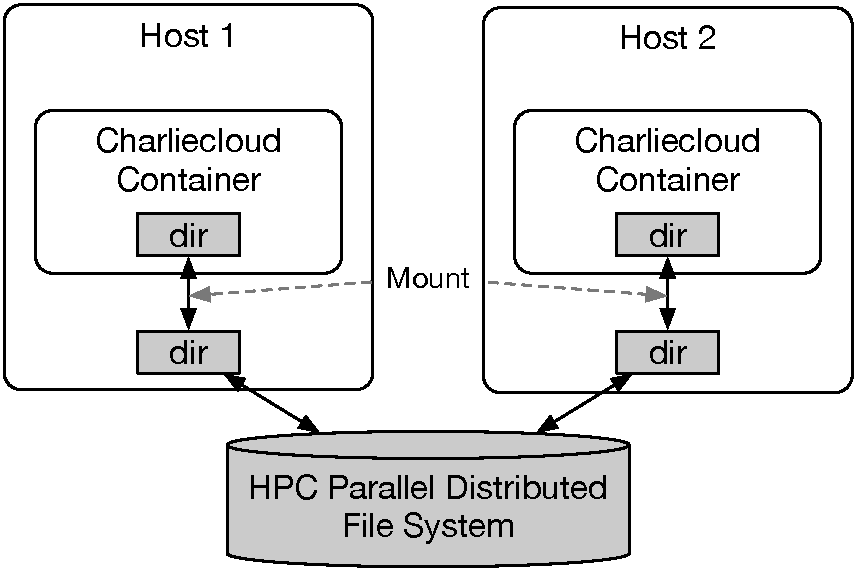
\includegraphics[width=0.4\textwidth]{figures/bee-cc.pdf}
    \caption{Shared Storage Design using Virtual IO}
    \label{bee-cc}
    \vspace*{-1em}
\end{figure}

When designing a \texttt{BEE backend}, one problem is identifying the suitable balance point between sharing and isolation of the runtime environment. Charliecloud offers comparable runtime isolation to Docker, that enables the user to pack all dependencies and tools in the image, avoiding additional application-specific configuration in the runtime environment. On the other hand, HPC applications usually require some degrees of data sharing: \textit{sharing via network} and \textit{sharing via storage}. 

\subsection{Network Design}
Sharing via network means processes running on different containers need to be able to share data via network. Charliecloud by default exposes all hardware network interfaces to its container runtime environment. Since HPC systems usually have interconnected networks between nodes, processes running in Charliecloud can communicate through the network interfaces on each node and get the benefits of any available network technology e.g., Infiniband. So, in \texttt{BEE-Charliecloud} we choose to the keep the default network settings. 

\subsection{Storage Design}
Sharing via storage is not natively supported by Charliecloud. By default each container only mounts the filesystem in the flattened input image. To enable sharing via storage, we use the \texttt{--bind} option  at container launch time to mount an user-specified host directory to a shared directory inside the container as mentioned in the user interface section. Since HPC systems usually have shared filesystem among nodes, processes can share data via the shared directory inside each container as shown in \textbf{Fig. \ref{bee-cc}} After each container is configured, \texttt{BEE-Charliecloud} automatically executes user's runscripts via the Charliecloud command \texttt{ch-run}. When initiating MPI parallel jobs, \texttt{BEE-Charliecloud} wraps \texttt{mpirun} command outside \texttt{ch-run} together with necessary MPI launching options. When deployed on HPC systems with Slurm resource manager, \texttt{BEE-Charliecloud} can interact with Slurm frontend to configure computing resources automatically. \textbf{Algorithm \ref{bee-cc-launch}} shows the launching logic of \texttt{BEE-Charliecloud}.

\begin{algorithm}
\caption{\texttt{BEE-Charliecloud} launching logic}
\label{bee-cc-launch}
\begin{algorithmic}[1]
\REQUIRE{Dockerized application (Docker image/Dockerfile)}
\REQUIRE{\texttt{BEE} configuration file (\texttt{beefile})}
\REQUIRE{Run scripts}
\STATE \texttt{pull/build\_docker(beefile)}
\STATE \texttt{flattened\_tar\_file $\leftarrow$ ch-docker2tar(docker\_image)}
\STATE \texttt{flattened\_filesystem $\leftarrow$ ch-tar2dir(flattened\_tar\_file)}
\STATE \texttt{compose\_ch-run\_options()}
\FOR{\textbf{each} \texttt{sequential run script} \textbf{in} \texttt{beefile} }
\STATE \texttt{slurm\_allocate\_resources()}
\STATE \texttt{ch-run(script)}
\ENDFOR
\FOR{\textbf{each} \texttt{parallel run script} \textbf{in} \texttt{beefile} }
\STATE \texttt{slurm\_allocate\_resources()}
\STATE \texttt{mpirun\_ch-run(mpi\_script)}
\ENDFOR

\end{algorithmic}
\end{algorithm}